A map's accuracy should mainly be determined by its purpose. It is usually taken to mean positional or locational accuracy. A map, which is strictly positional accurate, means that all features displayed have the correct scale and are precise in their location. However, thematic maps are often drawn at a very small scale, making it impossible to achieve such an accuracy. Generalisation impacts accuracy heavily. If generalisation with a focus on certain aspects of a map is applied, the map's accuracy will suffer \iacite{Tyner2010}.

According to \citeauthor{Tyner2010}, it is still possible to be rather truthful and accurate. This can be achieved by establishing following mindset: the thematic map, as well as all marks on it, are rather symbols than accurate representations. If this mindset is used while interpreting a thematic map, truthfulness and accuracy of a map can be defined as still showing the essence of geographic patterns and relationships \iacite{Tyner2010}.

The distinctness of map accuracy and map detail is important. The first generalisation method called selection already mentions this implicitly: accuracy refers to the amount of categories shown on the map, e.g. roads, rivers, lakes, etc., whereas detail relates to the amount of information shown for each category, e.g. only show rivers with a certain size \iacite{Tyner2010}.

As Chapter \ref{s:map-scale} on page \pageref{s:map-scale} already mentioned, the map scale is heavily dependent on the map projection. The true Figure of the earth is not a regular shape like a sphere or an ellipsoid. It has a separate shape, which is called geoid.
From a general point of view, every projection distorts the earth somehow, but the advantage of projection is, that any point can be exactly recreated at any given time, due to the fact, that the projection affects the whole earth.
A projection consists of four main properties:
\begin{enumerate*}[label={(\arabic*)}]
\item area,
\item form,
\item distance and
\item directions.
\end{enumerate*}
Every projection affects all its properties in some way. Some of them preserve area and form while distorting distances and directions \iacite{Snyder1987}.

In order to understand the following Section explaining different types of projections, some terms need to be explained first. \citeauthor{Snyder1987} divides the projection into three different ones \iacite{Snyder1987}:

\begin{enumerate}

\ditem{Conformal} \hfill \\
If a projection is conformal, it preserves local angles in the map. This can be thought of preserving the general shape of e.g. an island. Some parts of an island may get larger or smaller due to a conformal projection, but the recognisability of the island is still given.

\ditem{Loxodromes} \hfill \\
According to the Merriam-Webster Online Dictionary\footnote{See \href{http://www.merriam-webster.com/dictionary/rhumb\%2Bline}{http://www.merriam-webster.com/dictionary/rhumb\%2Bline}}, a loxodrome is also called rhumb line and can be defined as ``[\ldots] a line on the surface of the earth that follows a single compass bearing and makes equal oblique angles with all meridians''. A more practical example of loxodromes is to imagine a sailing route between two points. This line is shown as a straight line, as long as the intended course of the ship remains constant with respect to north.

\ditem{Equal-Area} \hfill \\
If a map bares the name equal-area, it means that it preserves area by distorting shapes.

\end{enumerate}

For most thematic maps irregularities of the earth's shape are ignored, as long as geodetic accuracy is not related to the purpose of the map \iacite{Snyder1987}. Figure \ref{fig:projections-base} on page \pageref{fig:projections-base} is in the subsections and helps to explain some major characteristics of the different types of projections. Every projection is only listed with its characteristics. These will not be discussed in detail, as it would go beyond the scope of this thesis.

\begin{figure}[!htb]
\centering
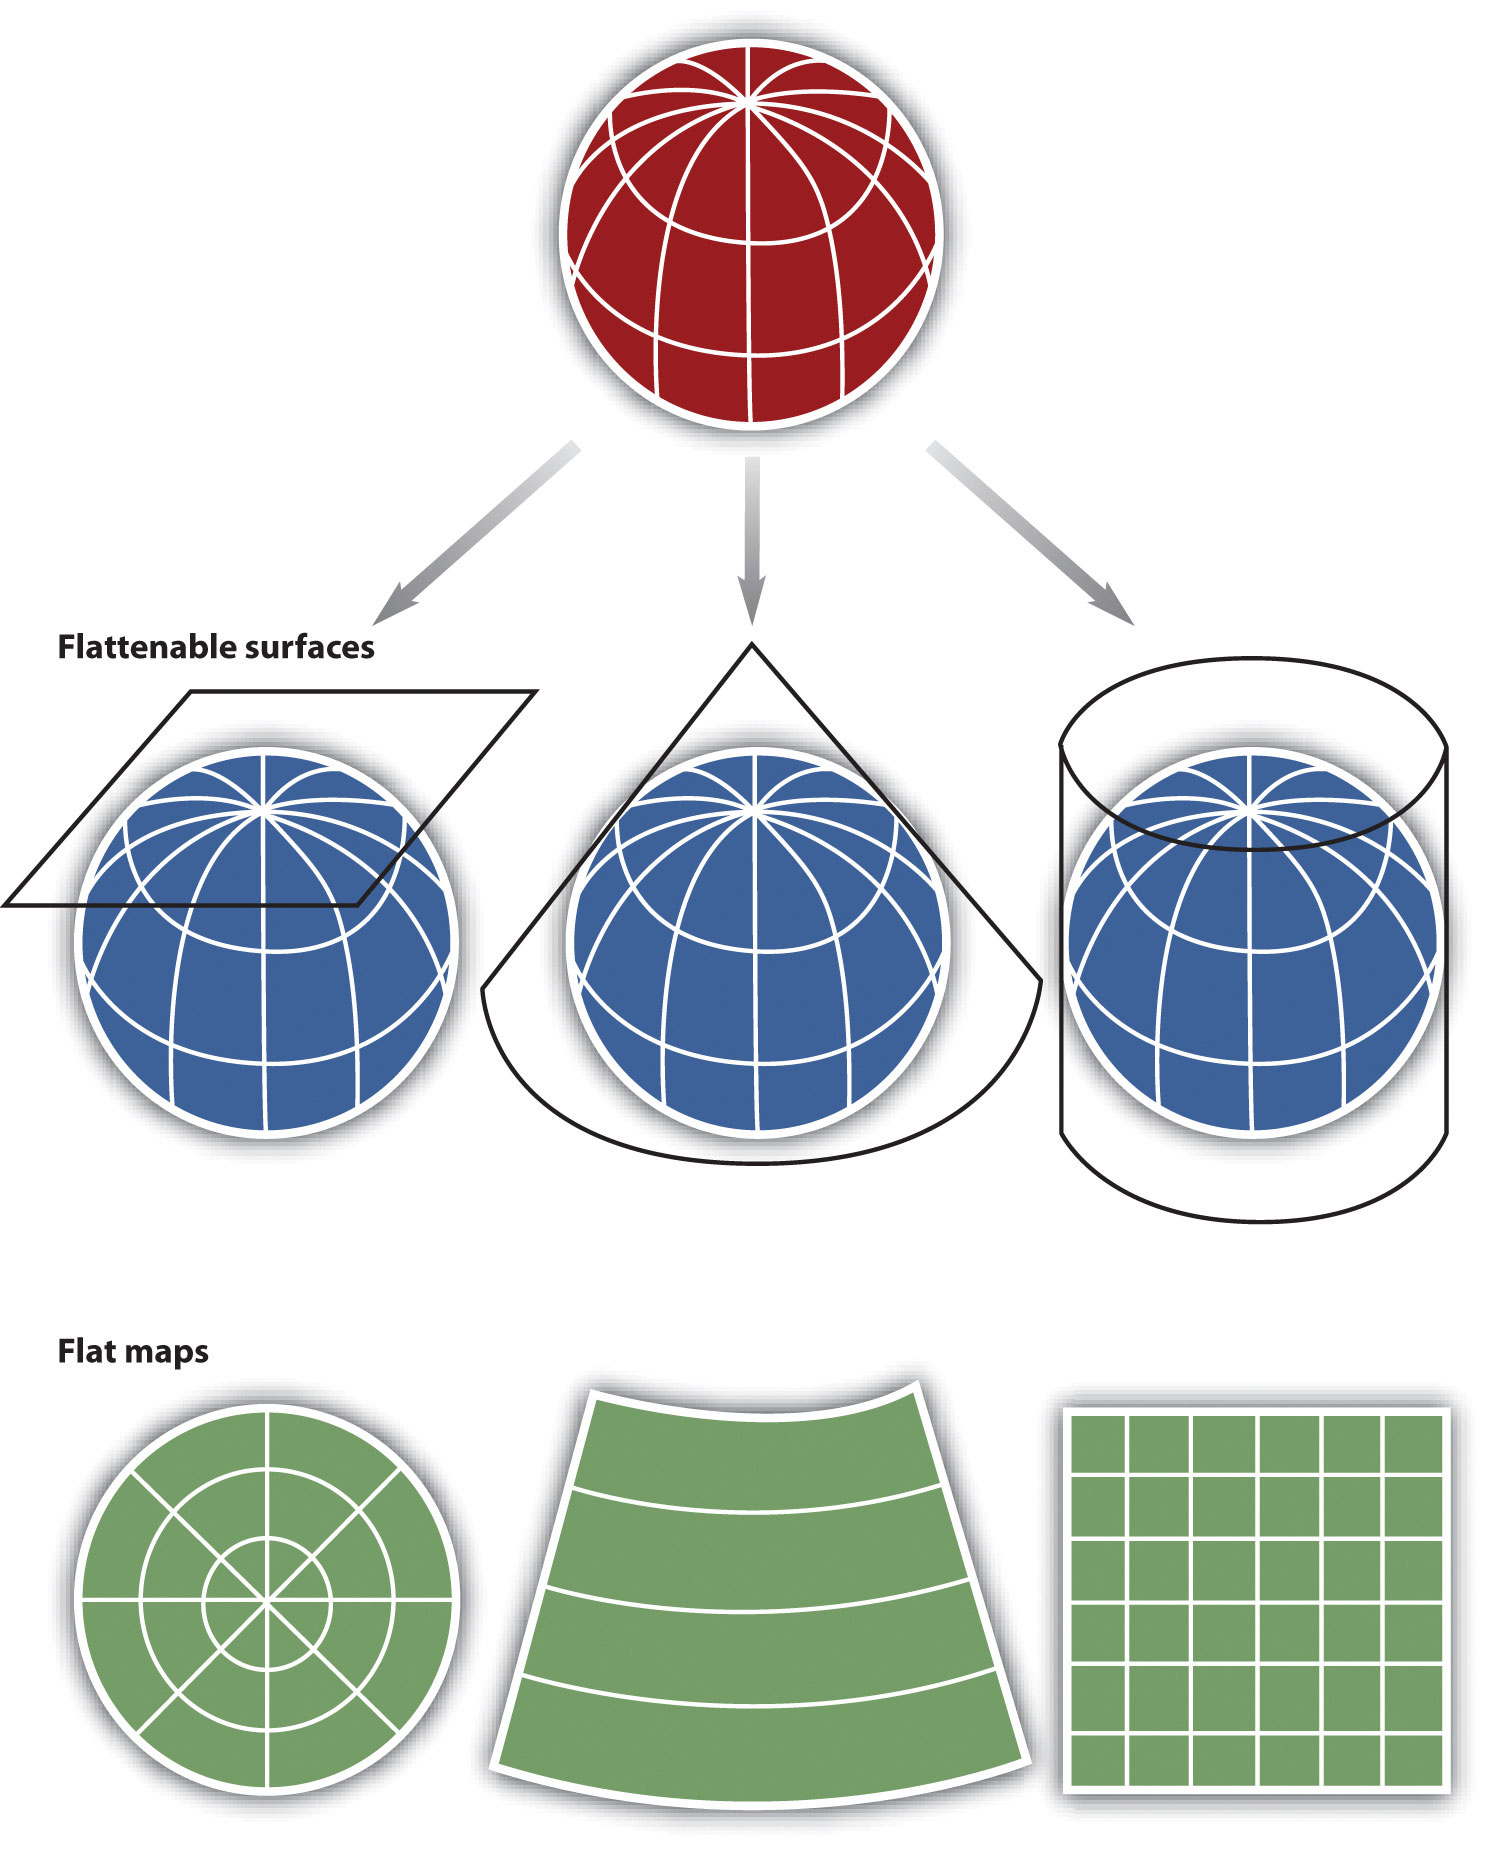
\includegraphics[height=5cm,keepaspectratio]{images/methods/projections/overview.jpg}
\caption[
    Projection of the earth onto the three major surfaces, Urldate: 08.2016 \newline
    \small\texttt{\url{http://images.flatworldknowledge.com/campbell/campbell-fig02_011.jpg}}.
]{Projection of the earth onto the three major surfaces.}
\label{fig:projections-base}
\end{figure}

\paragraph{Cylindrical Map Projections}
The main concept of cylindrical map projections consists ``[\ldots] of meridians which are equidistant parallel straight lines, crossed at right angles by straight parallel lines of latitude, generally not equidistant'' \iacite{Snyder1987}.
In general, cylindrical map projections can be thought of unrolling a cylinder which has been wrapped around a geoid, touching at the equator (see Figure \ref{fig:projections-base} on page \pageref{fig:projections-base}).
The primary use for this type of projection is to either map the complete world or for maps along narrow strips of a great circlel arc, such as the equator.

The following list will only feature two common projections accordingly to cylindrical projections with a short description taken from \citeauthor{Snyder1987} \iacite{Snyder1987}:

\begin{description}

\item[Mercator Projection] \hfill \\
It is a cylindrical, conformal projection where meridians are equally spaced straight lines, whereas parallels are unequally spaced straight lines. The scale of the map is only true along the equator and loxodromes are straight lines. The biggest distortion appears close to the poles. The major advantage according to \citeauthor{Snyder1987} is the navigational feature that loxodromes are straight lines \iacite{Snyder1987}. Figure \ref{fig:projections-mercator} on page \pageref{fig:projections-mercator} shows an example mercator projection of the earth.

\newpage
\item[Transverse Mercator Projection] \hfill \\
This projection is similar to the basic mercator projection except the main difference of being transverse in addition. The central meridian and each meridian 90 degrees east and west of the central meridian are straight lines. All other meridians and parallels are complex curves. The scale of the map is only true along the central meridian \iacite{Snyder1987}. Figure \ref{fig:projections-mercator-transverse} on page \pageref{fig:projections-mercator-transverse} illustrates the described characteristics.

\end{description}

\begin{figure}[!htb]
    \centering
    \subcaptionbox
    [
        Mercator projection, Urldate: 07.2016 \newline
        \small\texttt{\url{https://upload.wikimedia.org/wikipedia/commons/f/f0/MercNormSph.png}}.
    ]
    {
        Mercator projection.
        \label{fig:projections-mercator}
    }
  [.4\linewidth]
    {
        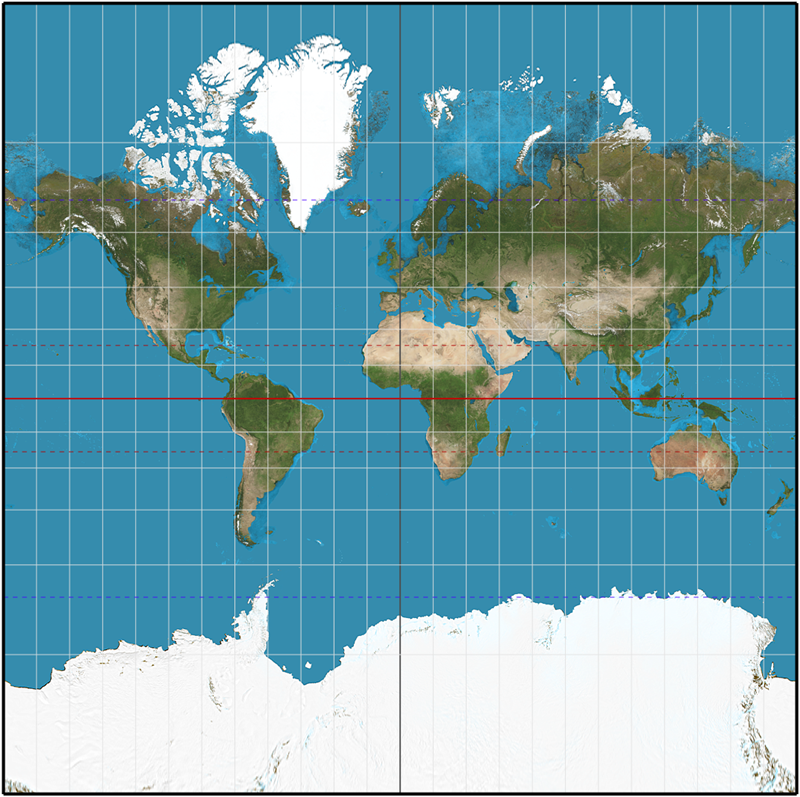
\includegraphics[width=0.4\textwidth,keepaspectratio]
        {images/methods/projections/mercator.png}
    }
    \qquad
    \subcaptionbox
    [
        Transverse mercator projection, Urldate: 07.2016 \newline
        \small\texttt{\url{https://upload.wikimedia.org/wikipedia/commons/1/15/MercTranSph.png}}.
    ]
    {
        Transverse mercator projection.
        \label{fig:projections-mercator-transverse}
    }
    [.4\linewidth]
    {
        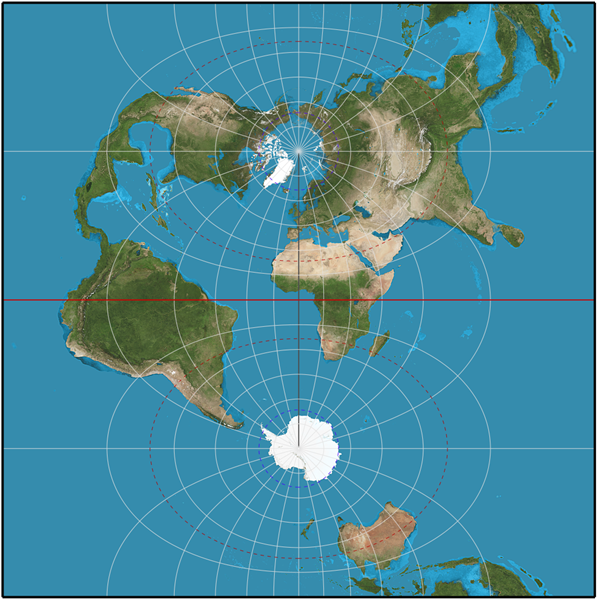
\includegraphics[width=0.4\textwidth,keepaspectratio]
        {images/methods/projections/mercator-transverse.png}
    }

    \caption{The mercator projection and its transverse counterpart.}
\end{figure}

\paragraph{Conic Map Projections}
Conic projections are preferred over cylindrical ones if the purpose of the map is to show a region for which the greatest areal extent is from east to west. This projection type makes use of ``[\ldots] arcs of concentric circles for parallels of latitude and equally spaced straight radii of these circles for meridians'' \iacite{Snyder1987}. The main distinctive feature is based on placing a cone on the top of a globe representing the earth (see Figure \ref{fig:projections-base} on page \pageref{fig:projections-base}).

The following list will only feature two common projections with a short description taken from \citeauthor{Snyder1987} \iacite{Snyder1987}:

\begin{description}
\item[Albers Equal-Area Projection] \hfill \\
\label{s:albers-equal-area-projection}
This projection, as seen in Figure \ref{fig:projections-albers-ea} on page \pageref{fig:projections-albers-ea}, is a conic, area-preserving one where parallels are unequally spaced arcs of concentric circles, whereas meridians are equally spaced radii of the same circles. It features no distortion in scale or shape along two standard parallels, normally, or along just one. Both poles are arcs of circles. The projection is used for regions with predominant east-west expanse \iacite{Snyder1987}.

\item[Equidistant Conic Projection] \hfill \\
Equidistant conic projection displays parallels, including poles, as arcs of concentric circles evenly spaced along the meridians. Like the albers equal-area projection, equidistant projection also displays meridians as equally spaced radii of the same circles and thereby cutting parallels at right angles. The scaling of the map is true along all meridians and along one or two standard parallels \iacite{Snyder1987}. Figure \ref{fig:projections-equidistant} on page \pageref{fig:projections-equidistant} shows similarities to the albers equal-area projection. The major distinction is the distortion of direction, area, and shape according to the distance from standard parallels.
\end{description}

\begin{figure}[!htb]
    \centering
    \subcaptionbox
    [
        Albers equal-area projection, Urldate: 07.2016 \newline
        \small\texttt{\url{https://upload.wikimedia.org/wikipedia/commons/1/1f/Albers_projection_SW.jpg}}.
    ]
    {
        Albers equal-area projection.
        \label{fig:projections-albers-ea}
    }
  [.4\linewidth]
    {
        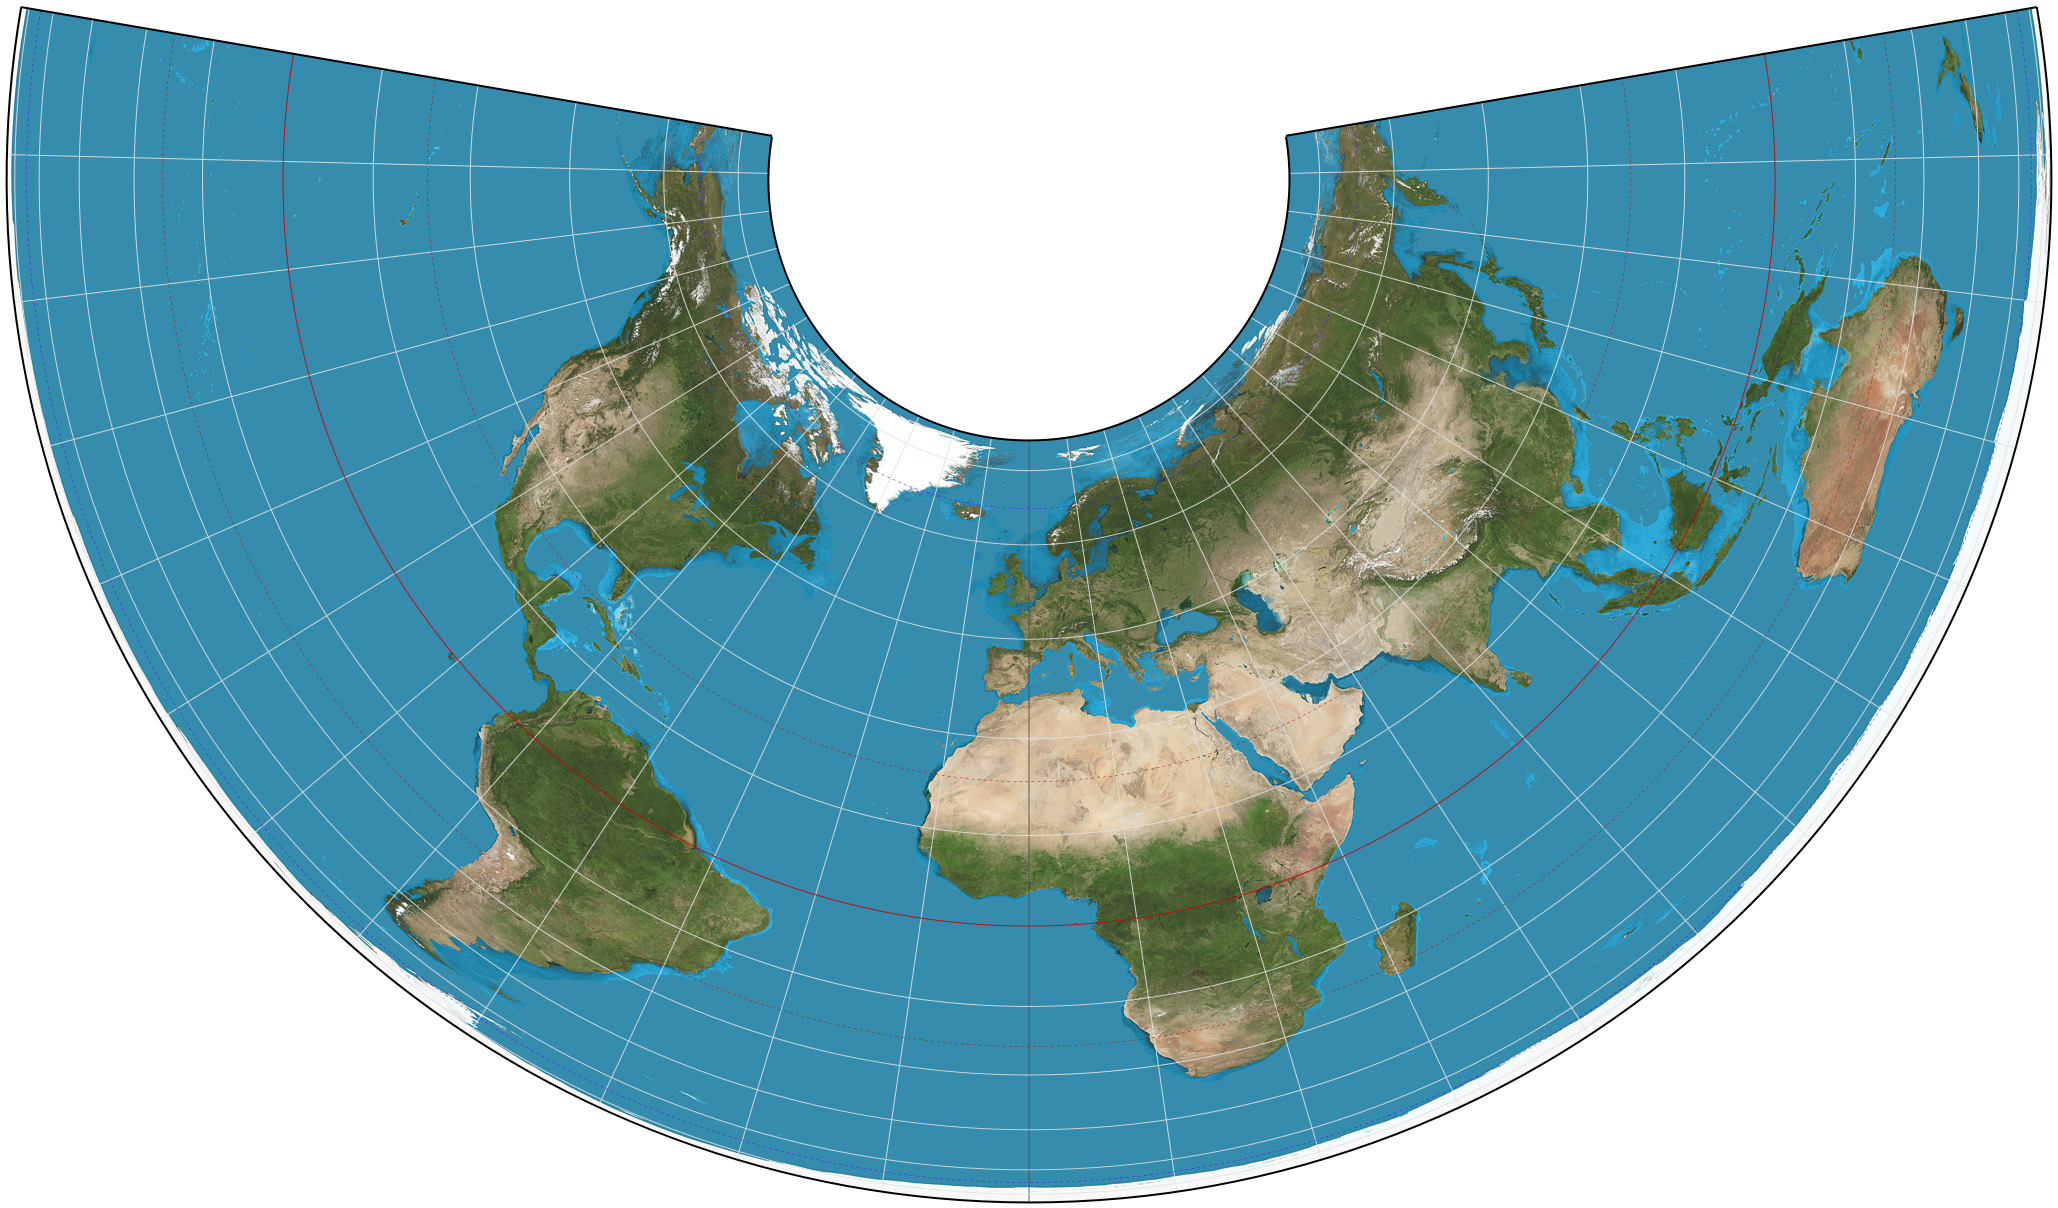
\includegraphics[width=0.4\textwidth,keepaspectratio]
        {images/methods/projections/albers.jpg}
    }
    \qquad
    \subcaptionbox
    [
        Equidistant conic projection, Urldate: 07.2016 \newline
        \small\texttt{\url{https://upload.wikimedia.org/wikipedia/commons/d/d8/Equidistant_conic_projection_SW.JPG}}.
    ]
    {
        Equidistant conic projection.
        \label{fig:projections-equidistant}
    }
    [.4\linewidth]
    {
        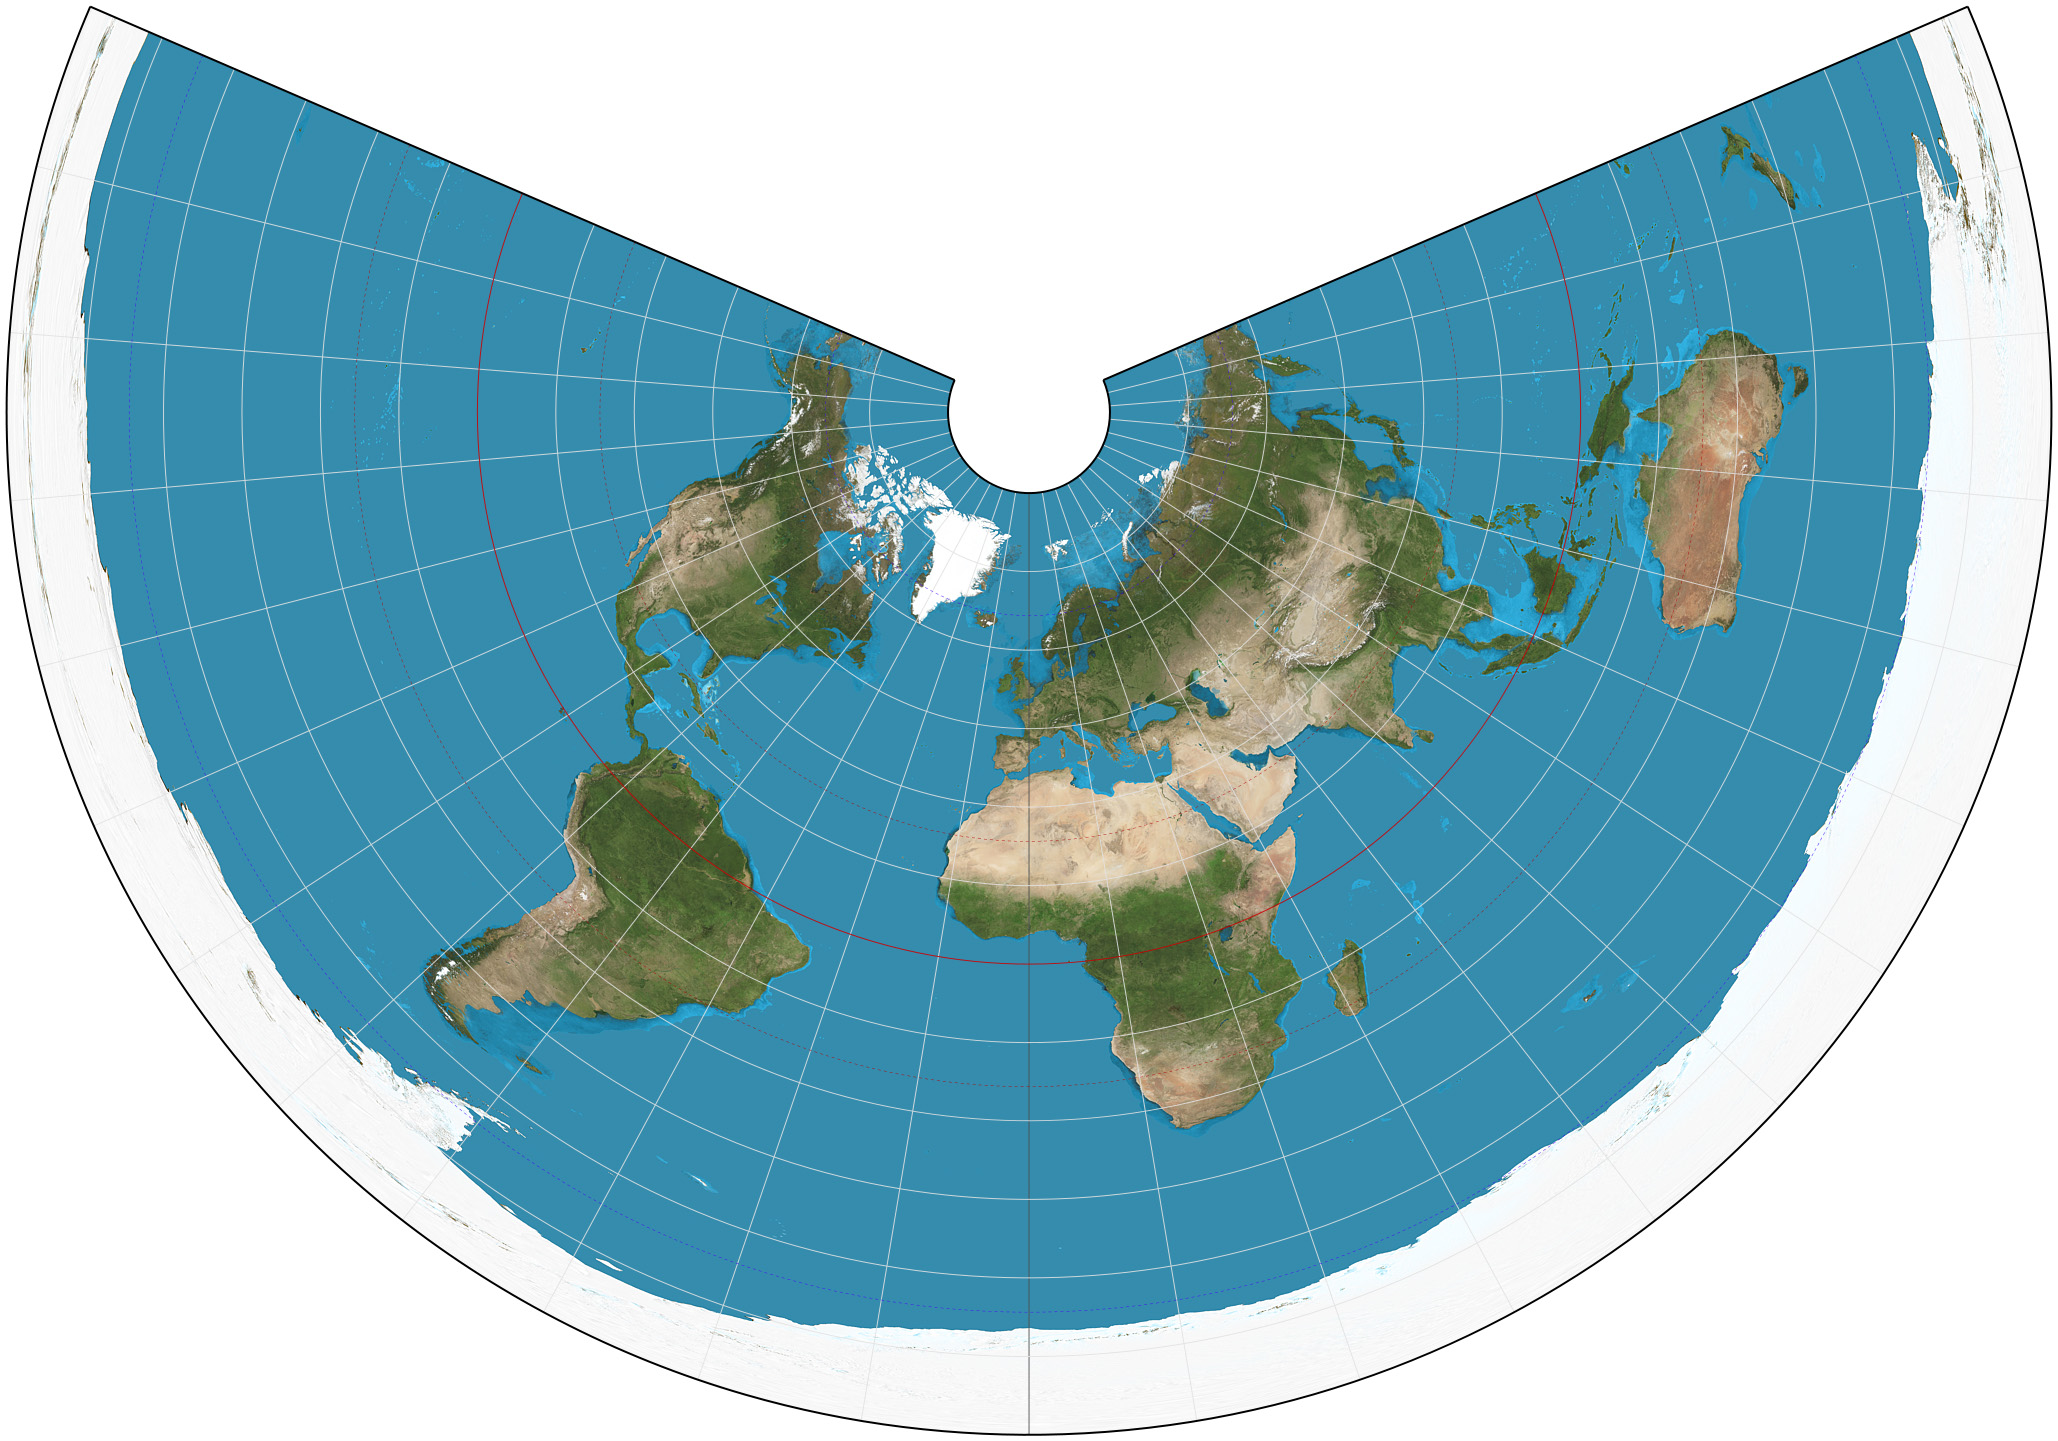
\includegraphics[width=0.4\textwidth,keepaspectratio]
        {images/methods/projections/equidistant.jpg}
    }

    \caption{Conic map projections.}
\end{figure}

\paragraph{Azimuthal and Related Map Projections}
Compared to cylindrical and conic projections which relate to cylinders and cones wrapped around the globe, azimuthal projections are mapped onto a plane. This plane usually is placed tangential at either pole, the equator, or any intermediate point. Each placement bears a different name and is called polar, equatorial and oblique aspects respectively. This type of projection attracted attention with the rise of radio transmission. This is due to the fact, that those type of projections show the direction from the centre of the projection to any other point on the map correctly. Figure \ref{fig:projections-azimuthal} on page \pageref{fig:projections-azimuthal} illustrates a polar azimuthal projection. All meridians are straight lines and radiate at their true angles from the centre, whereas parallels are concentric circles. Most azimuthal projections do not have standard parallels or standard meridians because each map has only one standard point. Azimuthals are not suitable for regions with predominant expanse in one direction because they will maximise distortion \iacite{Snyder1987}.

\begin{figure}[!htb]
\centering
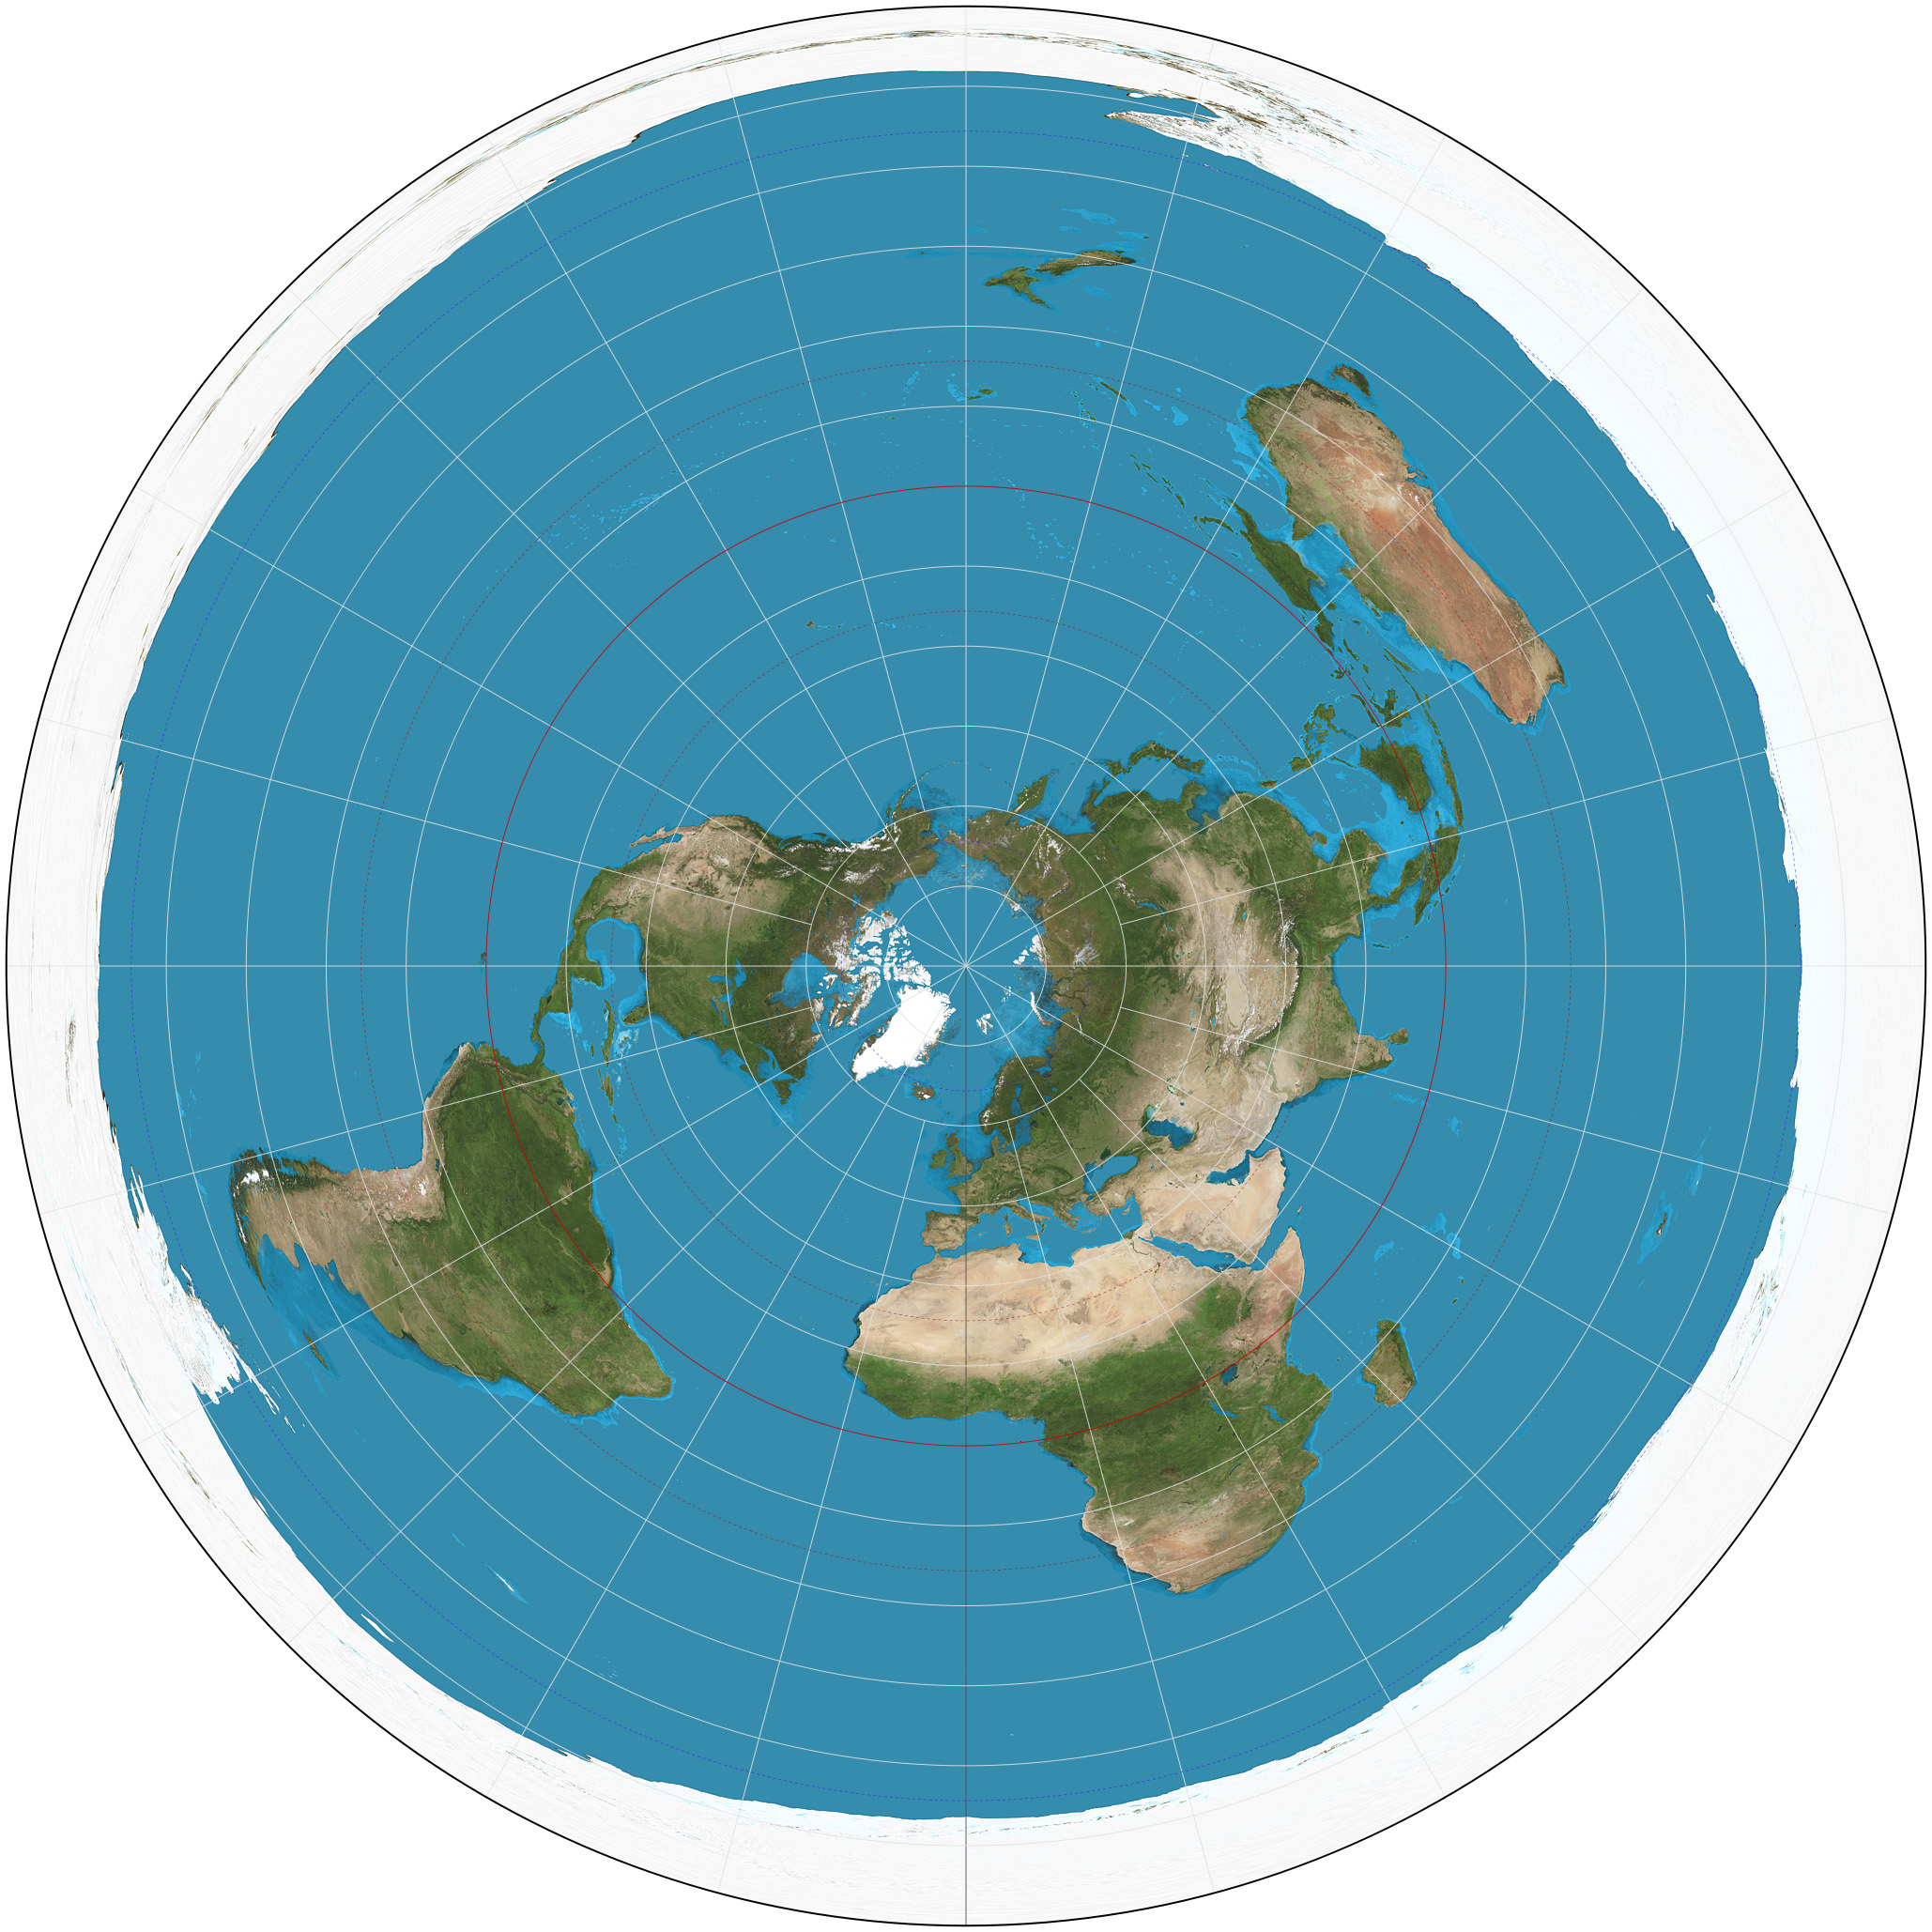
\includegraphics[height=5cm,keepaspectratio]{images/methods/projections/azimuthal.jpg}
\caption[
    Azimuthal projection, Urldate: 07.2016 \newline
    \small\texttt{\url{https://upload.wikimedia.org/wikipedia/commons/e/ec/Azimuthal_equidistant_projection_SW.jpg}}.
]{Azimuthal projection}
\label{fig:projections-azimuthal}
\end{figure}